\section{Dzia�anie programu}
Program sk�ada si� zasadniczo z dw�ch cz�ci. Pierwsz� z nich jest program napisany w jzyku c++, kt�rego zadaniem jest przetworzenie pliku z informacjami wej�ciowymi, oraz wygenerowanie rozwi�za�. Poprzez informacje wej�ciowe rozumiemy plik z zapisan� map�, na kt�rej program ma rozmie�ci� nadajniki. Mapa zawiera dozwolone miejsca dla nadajnik�w, oraz rozmieszczenie budynk�w oraz ich typy\footnote{Poprzez typy rozumiemy ilo�� os�b zamieszkuj�cy dany budynek}. Rozwi�zania, kt�re generuje program prezentuj� ko�cowe optymalne rozmieszczenie nadajnik�w na mapie, wraz z informacj� o ich type\footnote{Poprzez typ nadajnika rozumiemy jego zasi�g, oraz co si� z tym wi��e - kosztem danego nadajnika}.

\subsection{Processor}
Program \textsc{processor} jest rdzeniem naszego projektu, kt�ry w zamierzeniu mia� w jak naprostszy, oraz jak najszybszy spos�b wygenerowa� 
rozwi�zanie optymalne problemu. Program jest aplikacj� konsolow�, tak wi�c aby skorzysta� z niego samego (bez wykorzystania nak�adki GUI) nale�y
uruchomi� program w konsoli (cmd.exe w windows, b�d� w terminalu pow�oki linuks/unix). Program wywo�ujemy w spos�b nast�puj�cy:
\begin{verbatim}
processor --input=INPUT --silent --K=x --T=y --ALPHA=z
\end{verbatim}
Wszystkie parametry opr�cz pierwszego (input) s� opcjonalne. Poni�ej opis parametr�w programu:
\begin{itemize}
    \item input nazwa pliku wej�ciowego (mapy)
    \item silent - tryb bez dodatkowych komunikat�w oraz informacji - wykorzystywany przez nak�adk� GUI
    \item{K, T, ALPHA} parametry odpowiednio K - ilo�� iteracji, ALPHA - parametr algorytmu, T - ilo�� iteracji przez jak� dany element jest na 
          li�cie tabu
\end{itemize}


\subsection{GUI}
\subsubsection{Informacje og�lne}
Graficzny Interfejs U�ytkownika (GUI) zosta� napisany w j�zyku Java przy u�yciu komponent�w Swing i AWT. Zadaniem Interfejsu jest przyjazna dla u�ytkownika obs�uga programu "processor". Naszym celem by�o umo�liwienie bezproblemowej pracy programu w systemie Linux oraz Windows. Poniewa� interfejs jest napisany w Javie mo�na go uruchamia� w dowolnym systemie zawieraj�cym JRE 1.5.x. Nale�y oczywi�cie dysponowa� odpowiednim plikiem wykonywalnym procesora  (jako, �e jest pisany w C++).
\subsubsection{Okno g��wne}
Zrzut okna g��wnego znajduje si� na rysunku \ref{fig:mainWnd}:\\
\begin{figure}[!h]
  \centering
  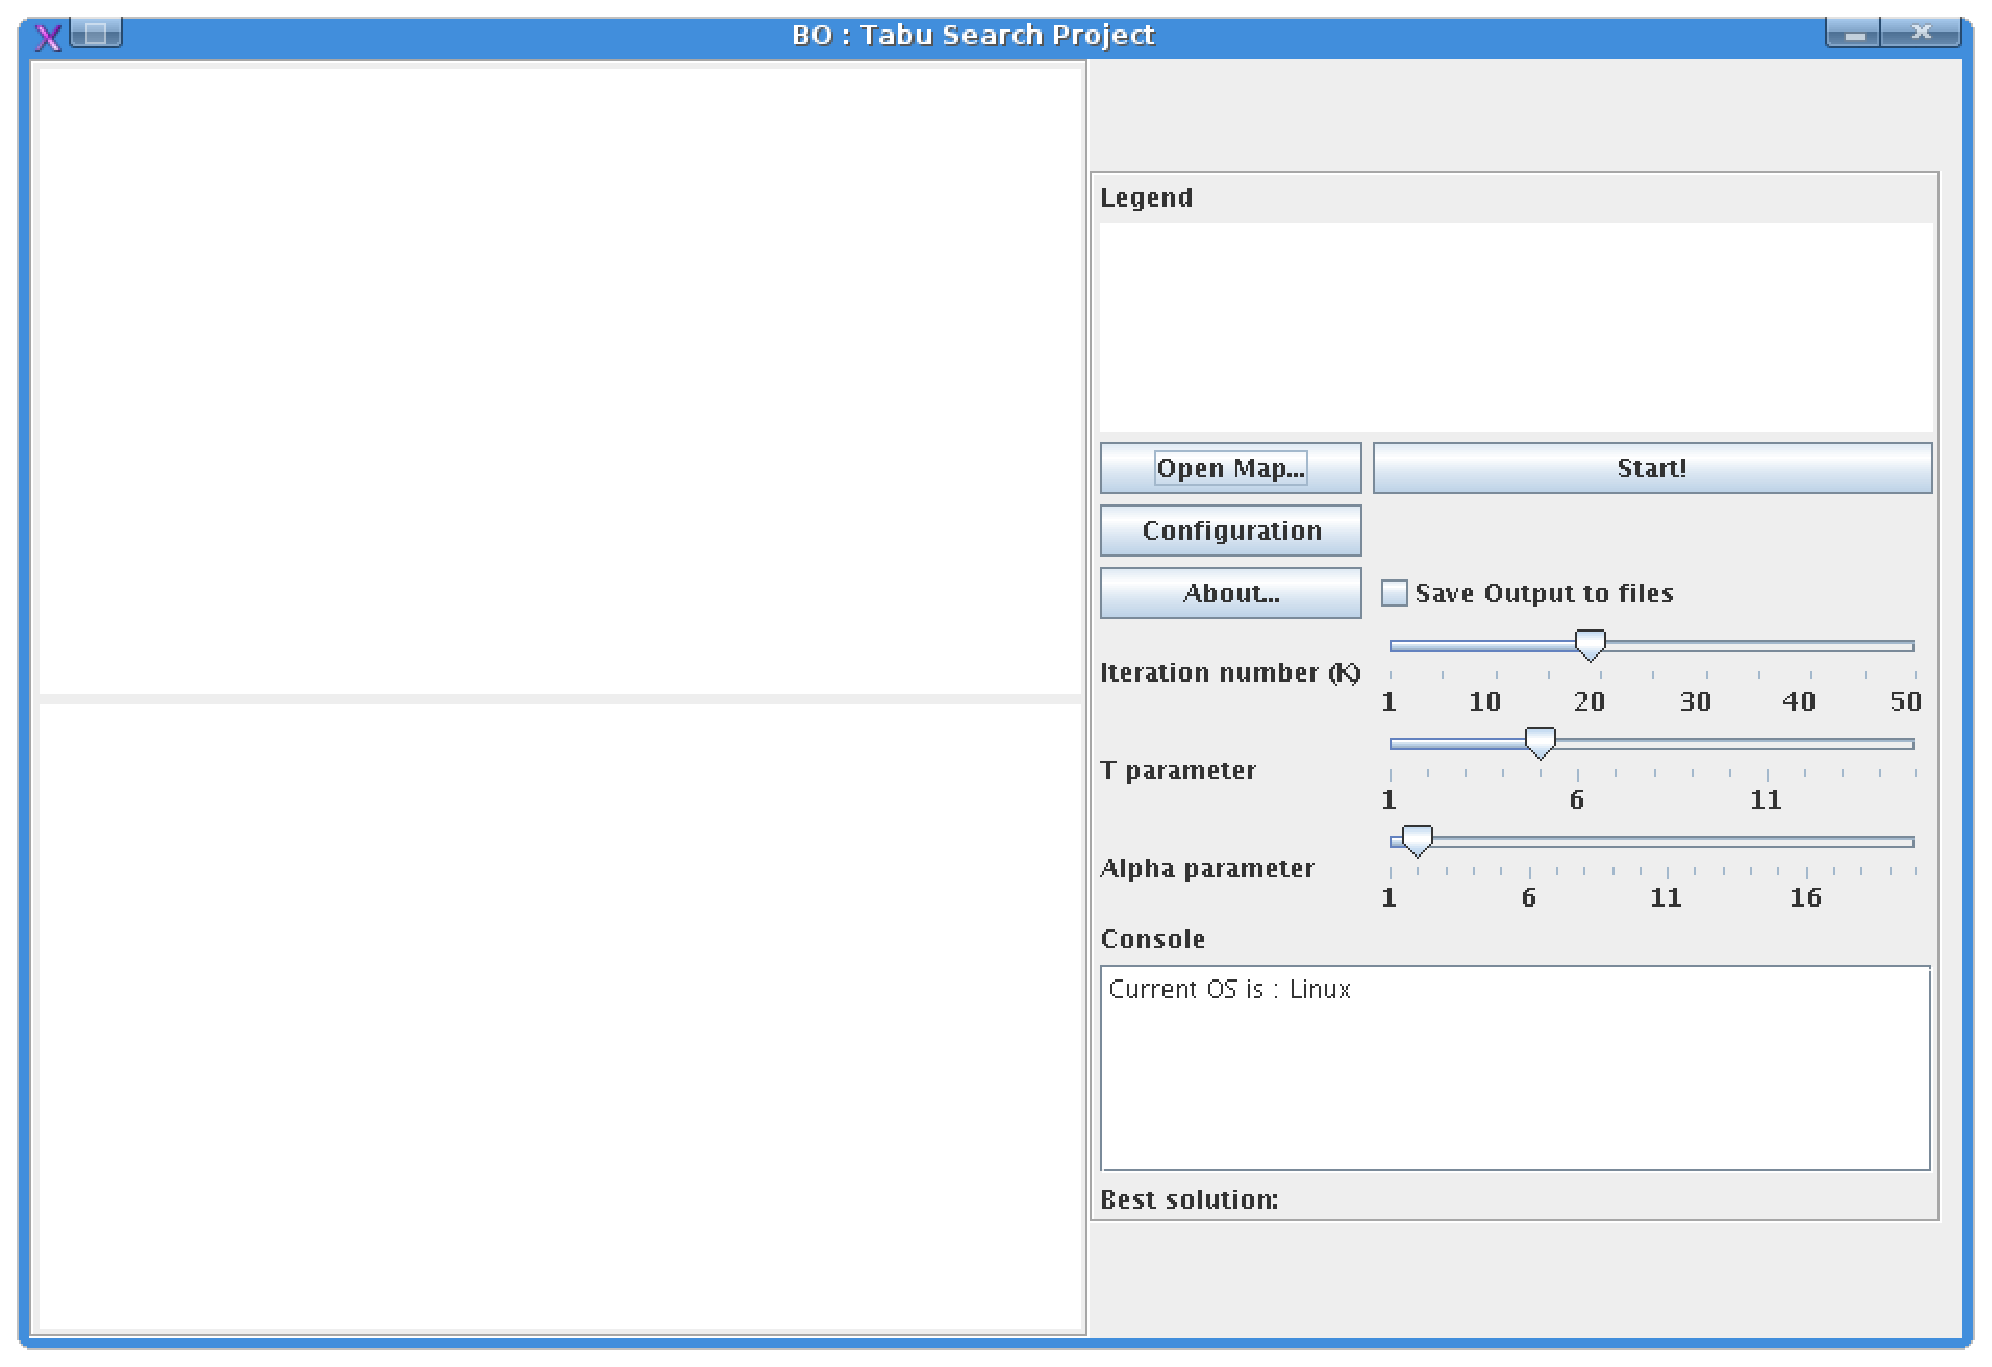
\includegraphics[width=0.75\textwidth]{./img/mainWnd.eps}
  \caption{G��wne okno programu}
  \label{fig:mainWnd}
\end{figure}
% 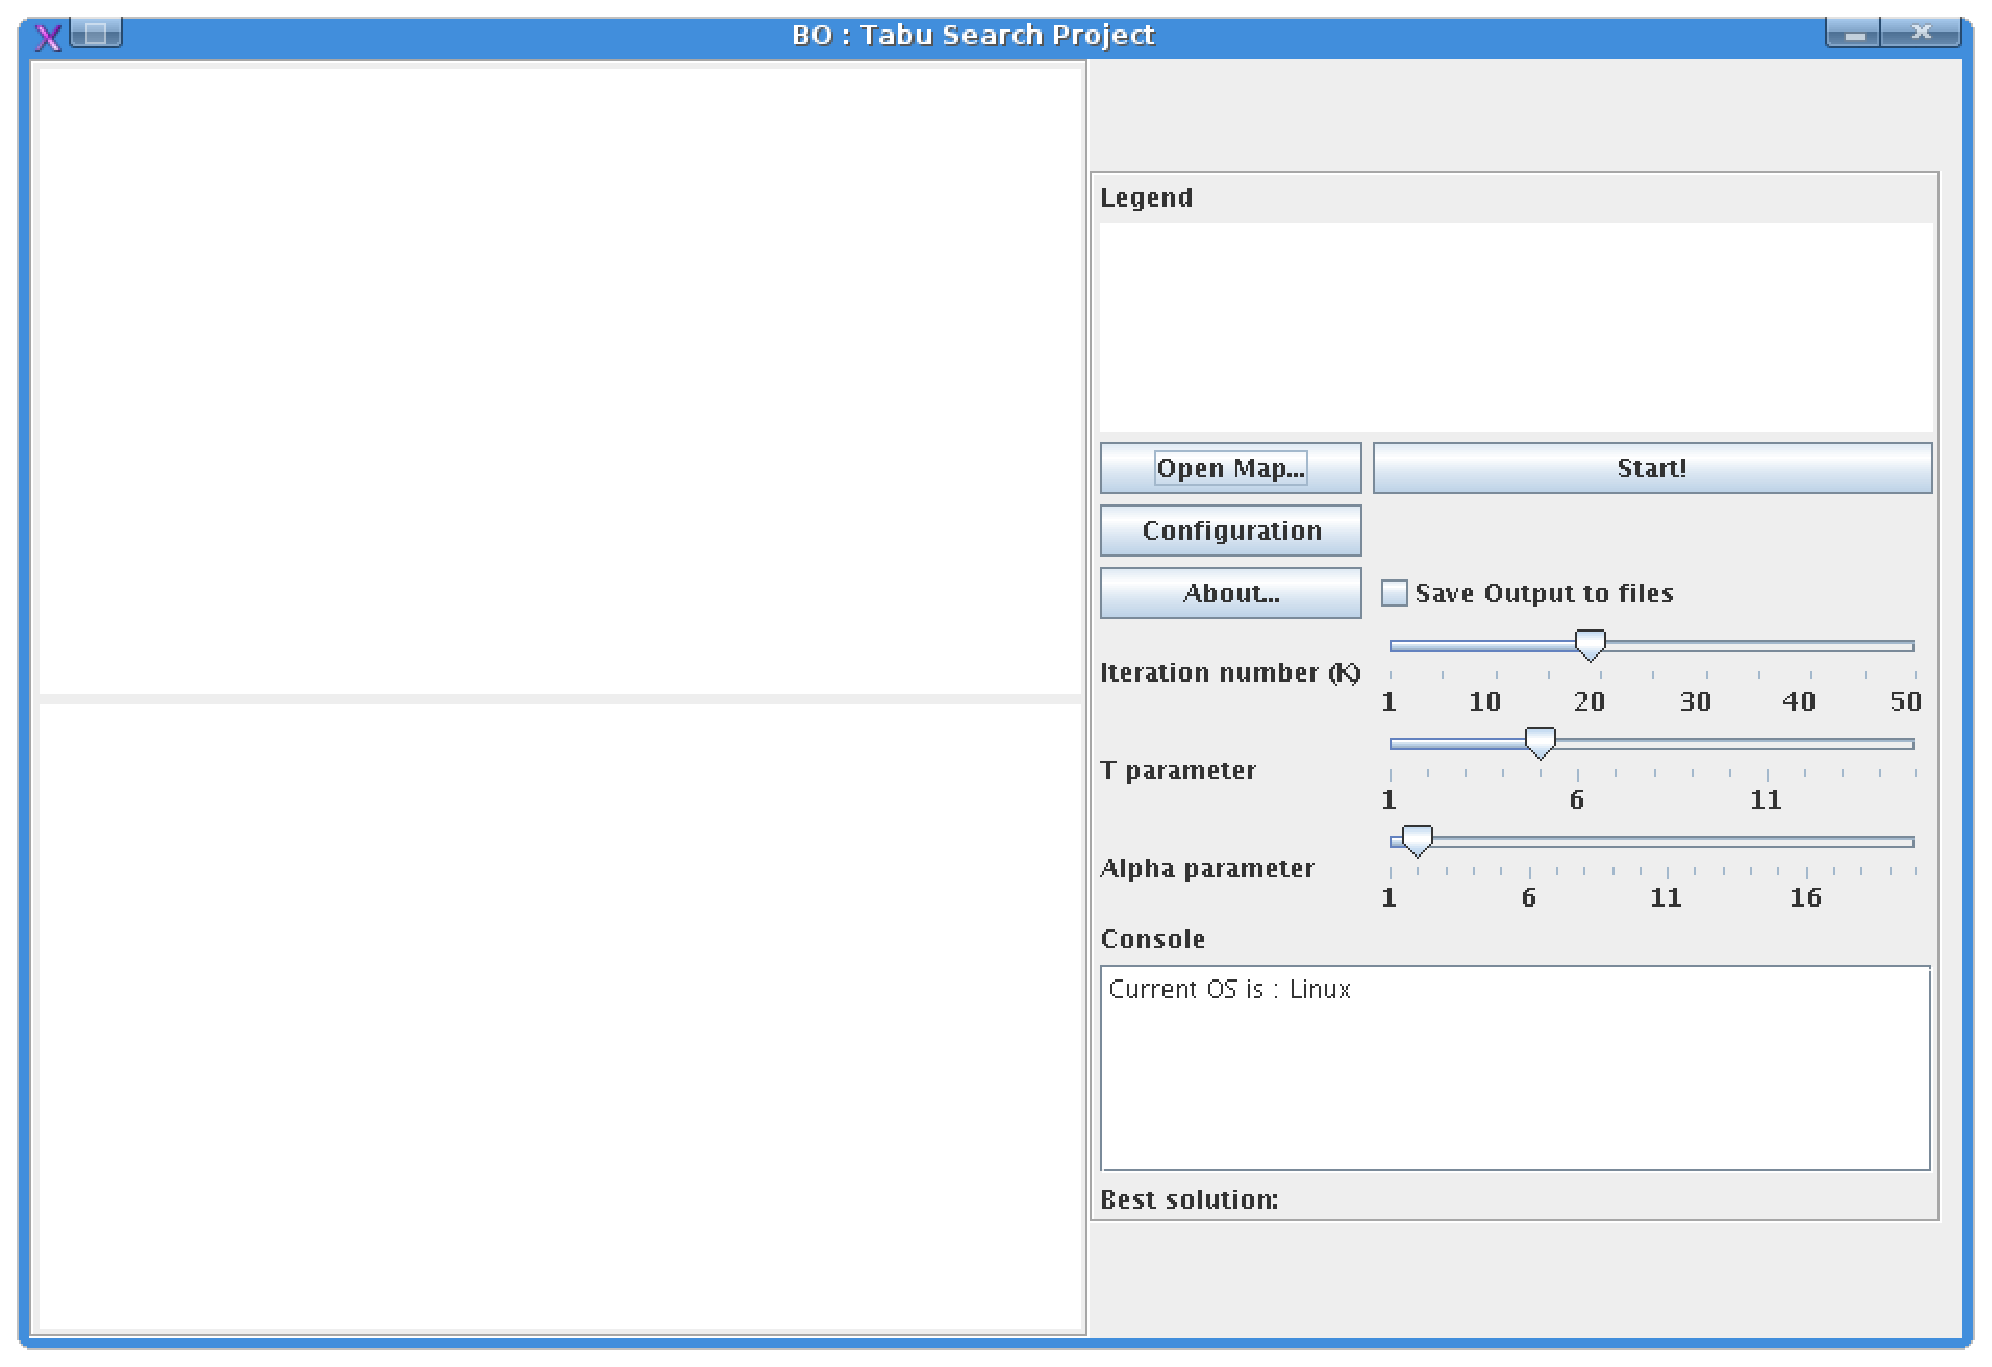
\includegraphics[width=1.0\textwidth]{./img/mainWnd.eps}\\[1cm]
Interfejs sk�ada sie z kilku podstawowych cz�ci: po lewej znajduj� si� obszary na kt�rych jest rysowane mapa i wykres funkcji celu. Po prawej znajduje si� legenda opisuj�ca map� ( przypisuje kolory do oznacze� budynk�w ) oraz przyciski steruj�ce dzia�aniem programu: \\
\begin{itemize}
  \item "Open Map..." - klikni�cie tego przycisku powoduje otwarcie okienka wyboru pliku zawieraj�cego map�. Za�adowanie pliku mapy jest niezb�dne do rozpocz�cia oblicze�. 

  \item "Configuration"- otwiera okno konfiguracji parametr�w (zyski z poszczeg�lnych typ�w budynk�w oraz opis anten: koszt i zasi�g). Program posiada pewne domy�ne parametry, wi�c konfiguracja nie jest obligatoryjna. Dok�adniejszy opis znajduje si� w dalszej cz�ci tej sekcji.

  \item "About" - otwiera okno opisuj�ce autor�w tego projektu

  \item "Save Output to files" - zaznaczenie tego pola pozwala na wybranie katalogu do zapisywania danych wyj�ciowych. Program zapisuje wyj�cie jako cztery pliki: 3 pliki PNG , zawieraj�ce map� wykres funkcji celu oraz legedn�, oraz jeden plik tekstowy w kt�rym znajduj� si� parametry z jakimi zosta�y wykonane obliczenia.

  \item "Start" przycisk kt�ry uruchamia obliczenia, lub je zatrzymuje je�eli zosta�y ju� rozpocz�te.
\end{itemize}

Ponadto na oknie g��wnym znajduj� si� r�wnie� suwaki do zmiany parametr�w: K, T, Aplha kt�re zosta�y opisane w poprzednich paragrafach.
\\
Na dole okna znajduje si� konsola na kt�r� s� wypisywane najwa�niejsze informacje o stanie dzia�ania programu. W niej pojawiaj� si� r�wnie� ostrze�enia o b��dach. Poni�ej konsoli znajduje si� etykieta na kt�rej wy�wietla si� informacja o najlepszym znalezionym rozwi�zaniu. \\
\subsubsection{Konfiguracja}
Okno konfiguracji znajduje si� na obrazie \ref{fig:confProfit}.
\begin{figure}
  \centering
  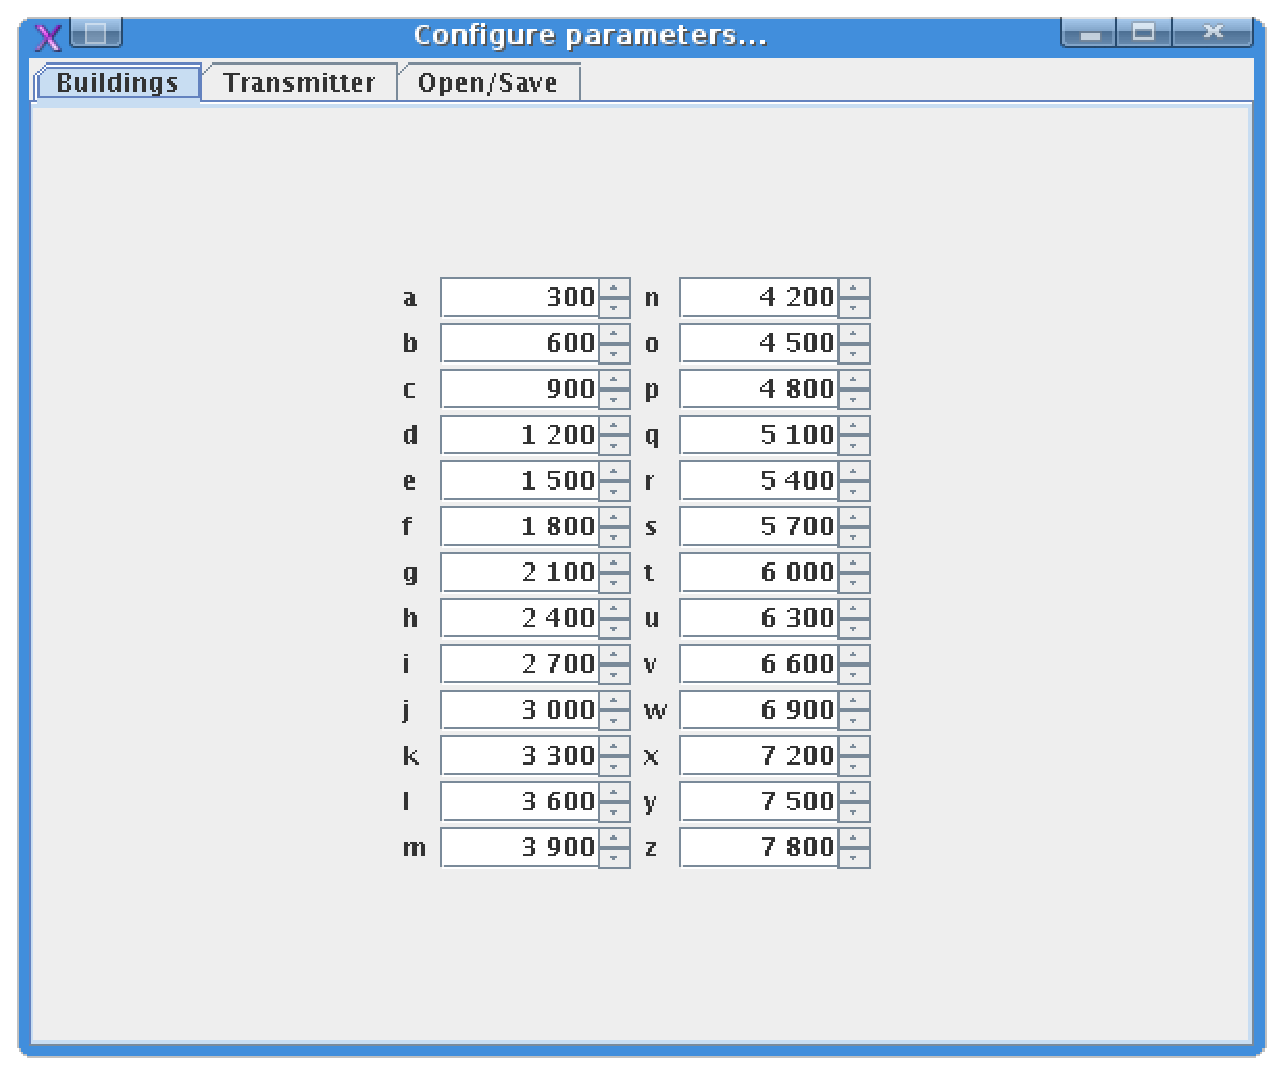
\includegraphics[width=0.75\textwidth]{./img/confWndProfit.eps}
  \caption{Okno konfiguracji: Edycja budynk�w}
  \label{fig:confProfit}
\end{figure}
% 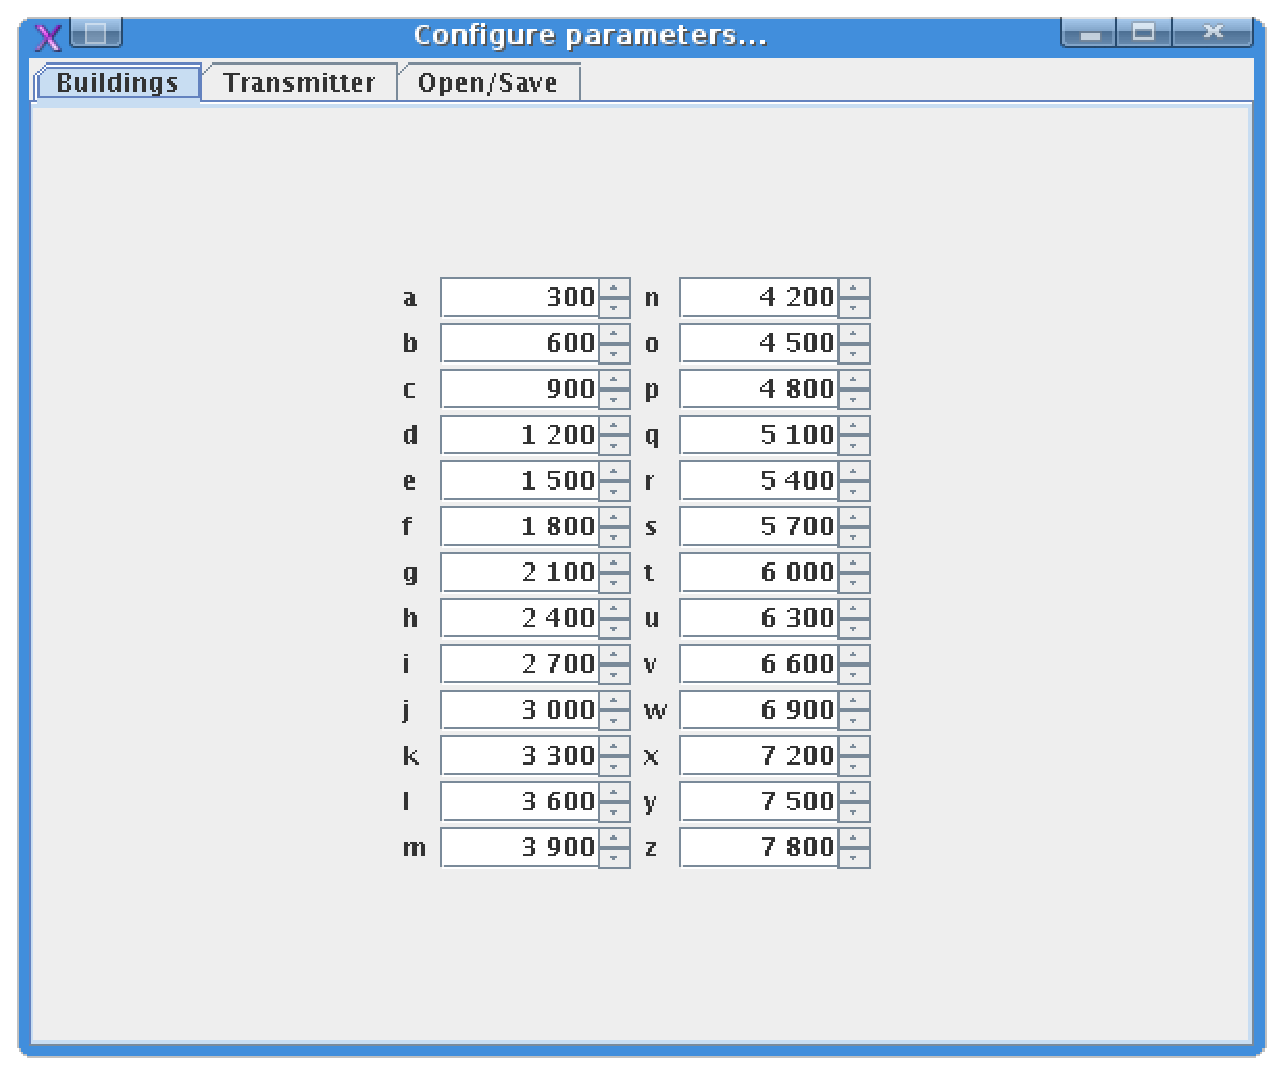
\includegraphics[width=1.0\textwidth]{./img/confWndProfit.eps}\\[1cm]
Tutaj pokazana jest konfiguracja zysk�w z obj�cia danego budynku zasi�giem. W naszym projekcie rozr�niamy budynki oznaczaj�c je literami alfabetu 'a' - 'z' (bez polskich liter). Ka�demu rodzajowi budynku mo�na przyporz�dkowa� dowolny nieujemny zysk. Przek�ada si� to na wygl�d mapy i oczywi�cie rezultat oblicze�.\\
Kolejn� zak�adk� jest konfiguracja anten pokazana na obrazie \ref{fig:confTrans}
\begin{figure}
  \centering
  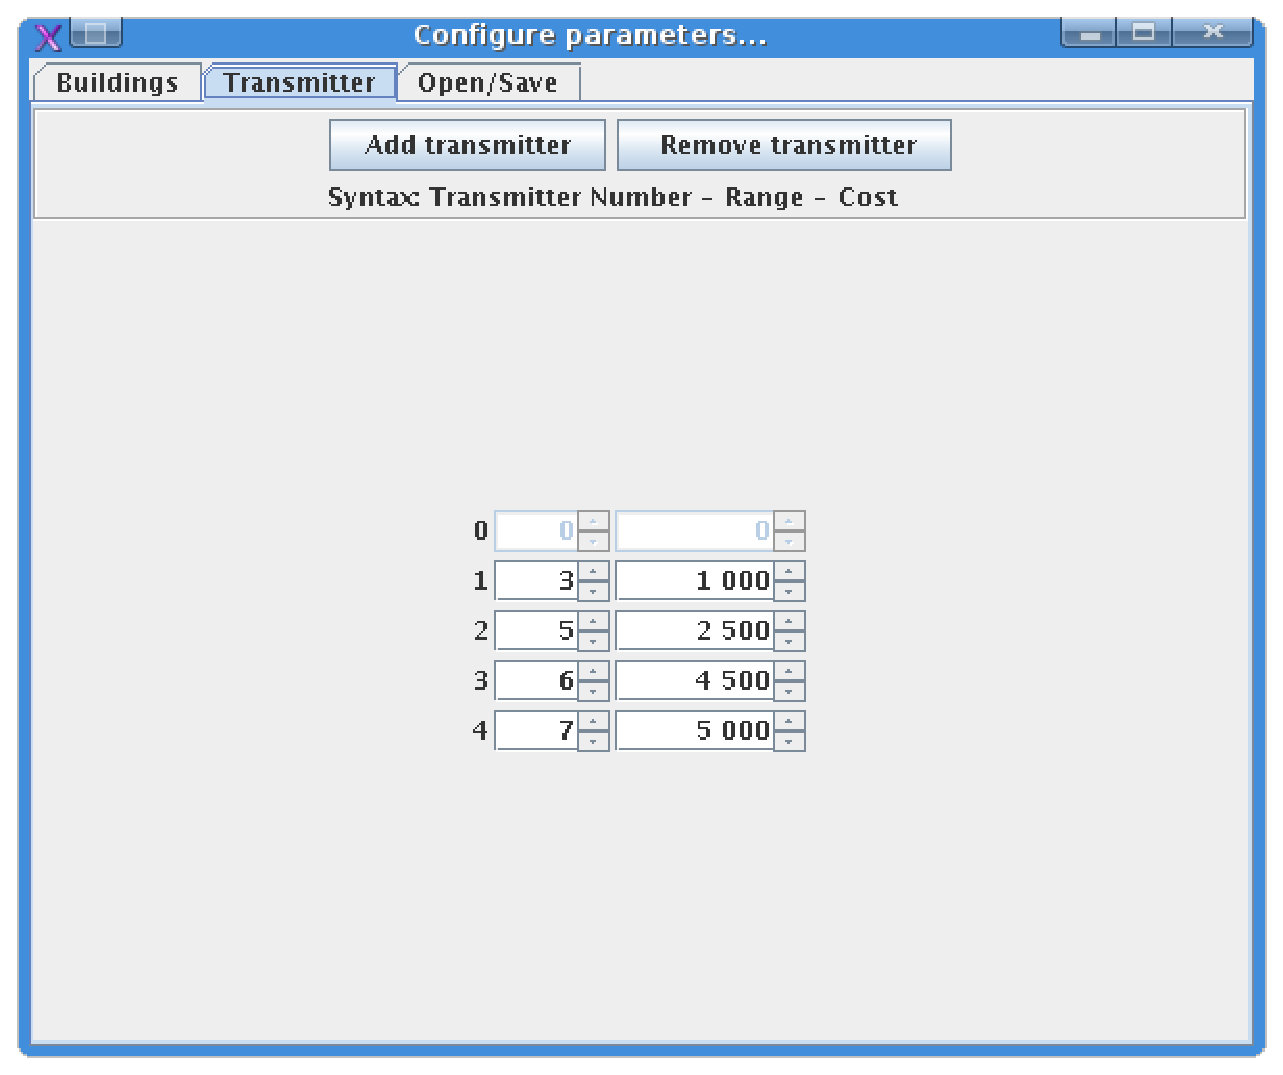
\includegraphics[width=0.75\textwidth]{./img/confWndTransEdit.eps}
  \caption{Okno konfiguracji: Anteny}
  \label{fig:confTrans}
\end{figure}
% 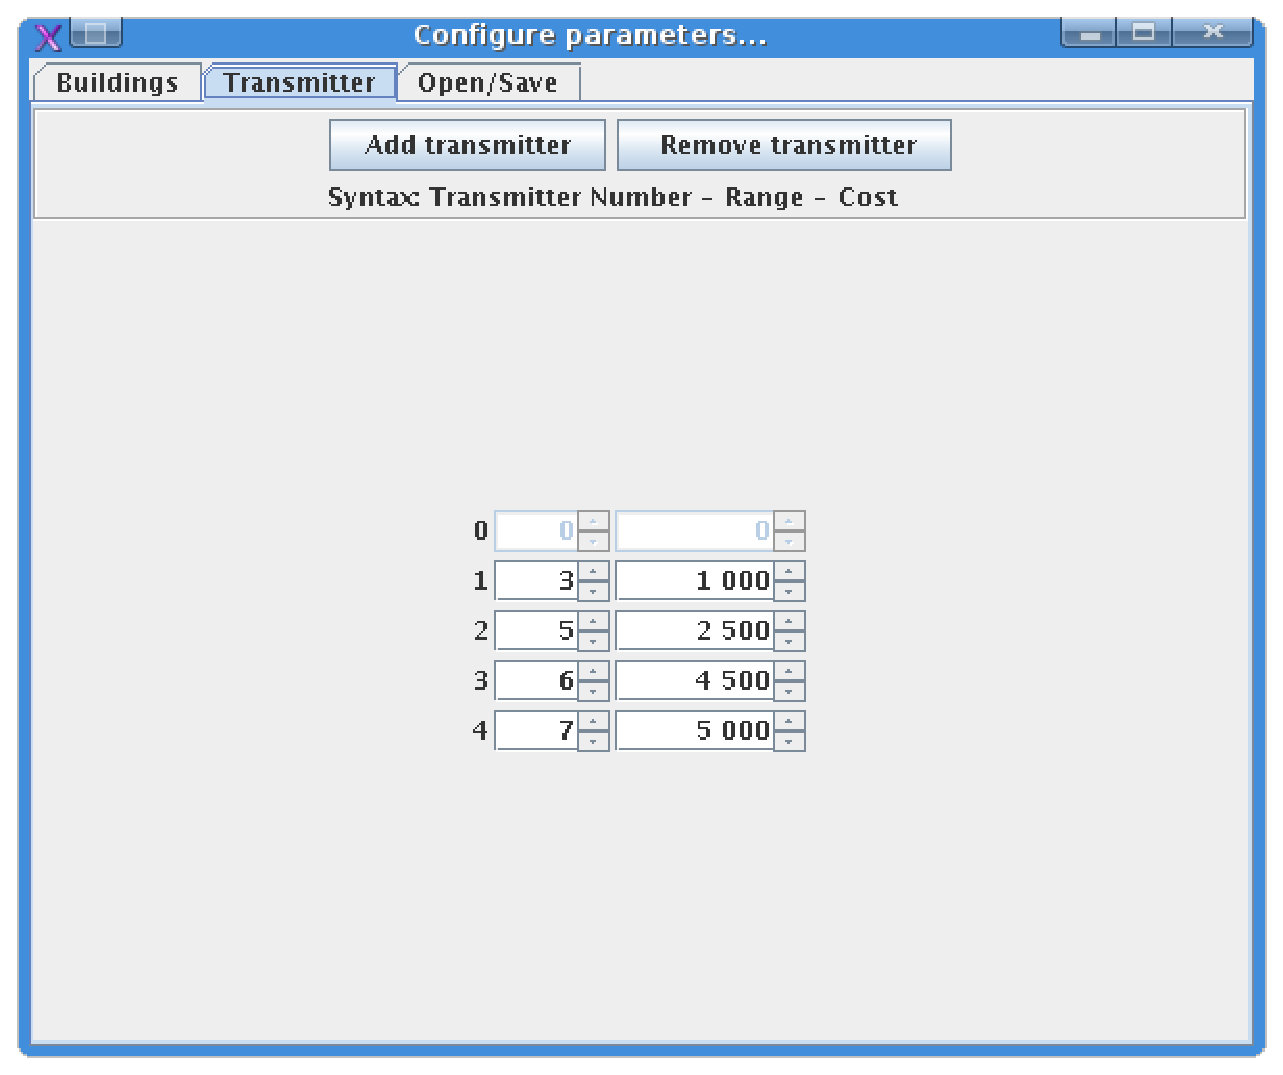
\includegraphics[width=1.0\textwidth]{./img/confWndTransEdit.eps}\\[1cm]
Klikni�cie na przycisk "Add transmitter" powoduje dodanie nowej anteny do listy. Ka�d� anten�, opr�cz zerowej, mo�na edytowa� tzn. ustala� jej zasi�g oraz koszt postawienia. Pierwsze pole odpowiada za zasi�g, a drugie za koszt.\\ Klikaj�c na przycisk "Remove transmitter" usuwamy anten� z listy. Nie mo�na usun�� tylko anteny "zerowej".
Ostatnia zak�adka s�u�y do zatwierdzenia konfiguracji, anulowania zmian, zapisania jej do pliku lub otwarcia istniej�cej zapisanej konfiguracji, zrzut ekranu z t� zak�adk� znajduje si� na obrazie \ref{fig:confFiles}\\
\begin{figure}
  \centering
  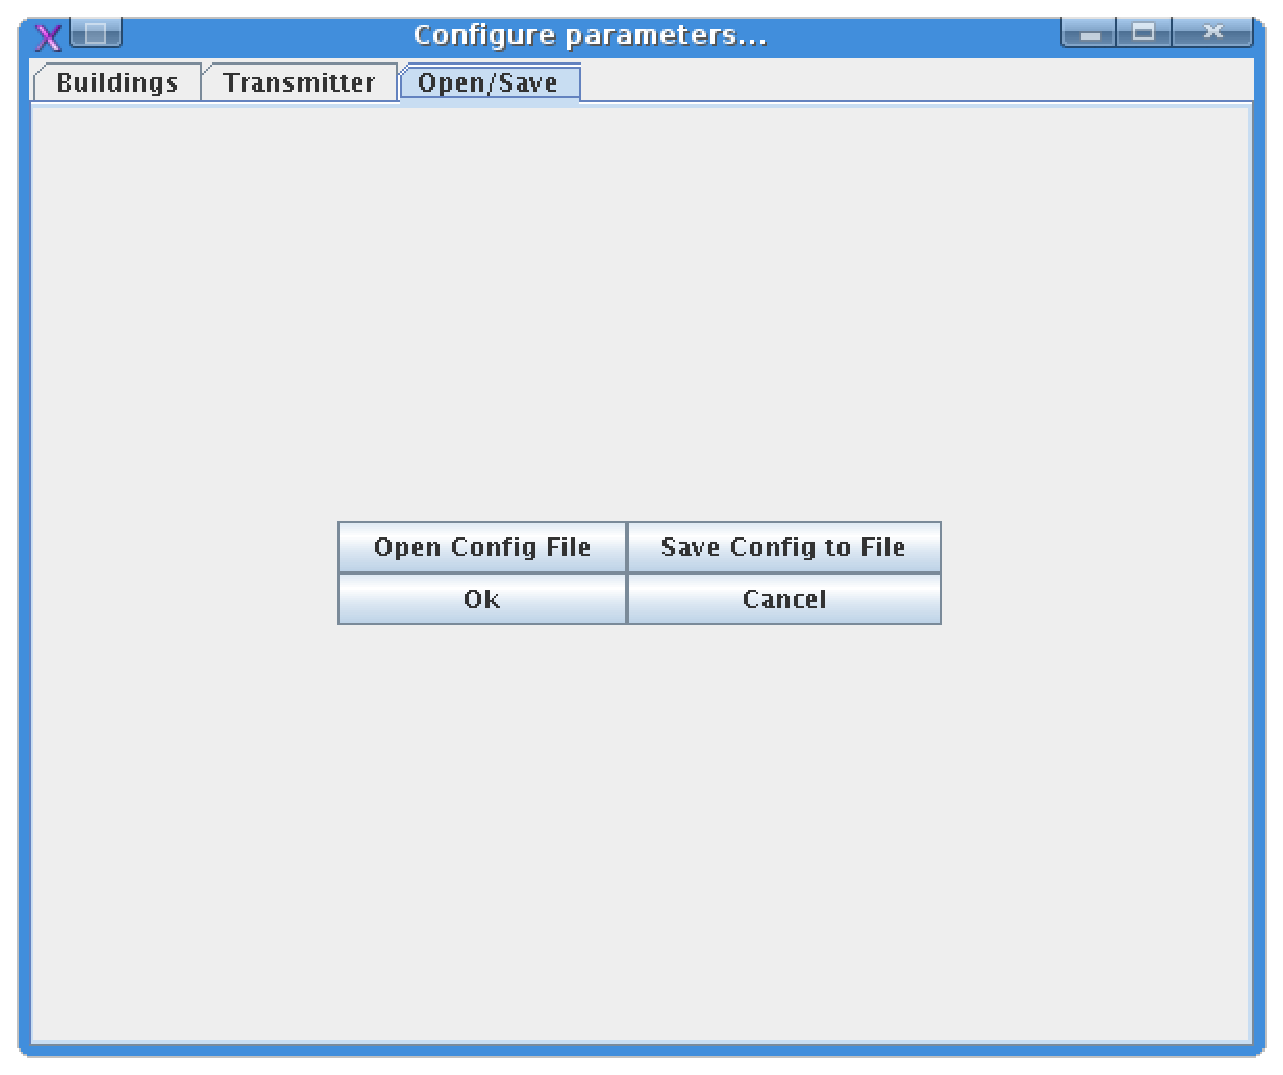
\includegraphics[width=0.75\textwidth]{./img/confWndFiles.eps}
  \caption{Okno konfiguracji: Otwieranie i zapisywanie konfiguracji}
  \label{fig:confFiles}
\end{figure}
% 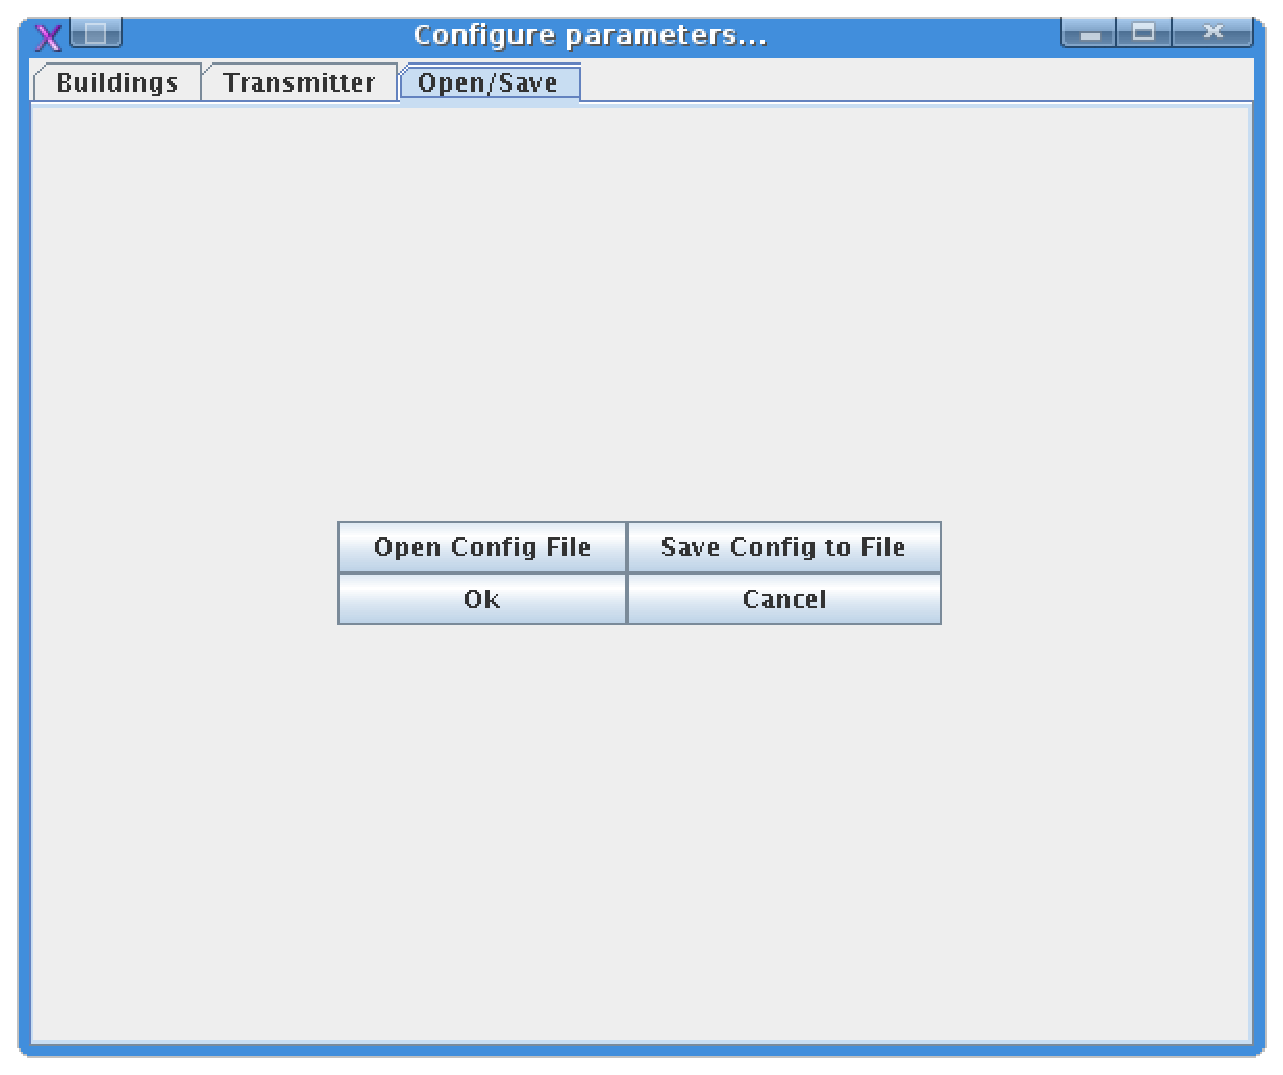
\includegraphics[width=1.0\textwidth]{./img/confWndFiles.eps}\\[1cm]
\subsubsection{Dzia�anie}
Pierwszym krokiem jest wczytanie mapy. Jest ona nast�pnie parsowana i na tej podstawie jest rysowana graficzna jej reprezentacja. Uruchomienie procesu obliczeniowego odbywa si� przez wci�ni�cie przycisku "Start". Powoduje to utworzenie nowego w�tku, w kt�rym jest wywo�ywany program "processor". Po jego zako�czeniu GUI analizuje jego wyj�cie i przetwarza je na obraz rozwi�zania (tzn zaznaczenie wybranych nadajnik�w oraz obrysowanie ich zasiegu) oraz rysuje wykres funkcji celu dla kolejnych iteracji. \\ Je�eli nie zosta�a zmieniona domy�nla konfiguracja to program korzysta z niej i nie przekazuje �adnej informacji jej dotycz�cej do "processora". W przeciwnym przypadku u�ytkownik musi najpierw zapisa� konfiguracj� do pliku, aby mog�a zosta� przekazana do procesu obliczeniowego.\\
Je�eli u�ytkownik zaznaczy� opcj� zapisu wyj�cia do pliku to zostan� wygenerowane pliki we wskazanym folderze. Generowane s� nast�puj�ce pliki o sk�adni:
\begin{itemize}
  \item \textit{<input\_file>\_graph.png} - obraz funkcji celu;
  \item \textit{<input\_file>\_map.png} - wizualizacja mapy;
  \item \textit{<input\_file>\_legend.png} - plik z obrazem legendy;
  \item \textit{<input\_file>\_config.txt} - plik tekstowy z informacj� o konfiguracji z jak� dane wej�ciowe by�y przetwarzane;
\end{itemize}
<input\_file> to nazwa pliku wej�ciowego (mapy).\\

